\subsection{Dateikonzept} \label{json_config_files}
Für das Dateikonzept wurden drei Dateitypen auf Basis von \acs{json} Dateien entwickelt. Abbildung \ref{fig:vereinfachter_aufbau_dateikonzept} dient dem besseren Verständnis des Dateikonzepts. Hauptsächlich zeigt diese einen vereinfachten Aufbau der Komponenten, die von der Firma Bösch zur Entwicklung einer \acs{rltanzeige} bereitgestellt wurden, und die dazugehörigen Konfigurationsdateien. Die \acs{rltanzeige} selbst ist über den Bus mit einem Ventilator von ebm-papst sowie einem QBM9711 von Siemens verbunden. Der Ventilator verfügt lediglich über integrierte Sensorik. Der QBM9711 hingegen verfügt über zwei integrierte Luftdruck-Sensoren (interne Ports 1 und 2), zwei (an die Ports Analog Input 1 und 2) extern angeschlossene Temperatursensoren, eine (an den Port Analog Output 1) extern angeschlossene Klappe und ein (an den Port Analog Output 2) extern angeschlossenes Relais.


\begin{figure}[H]
	\centering
	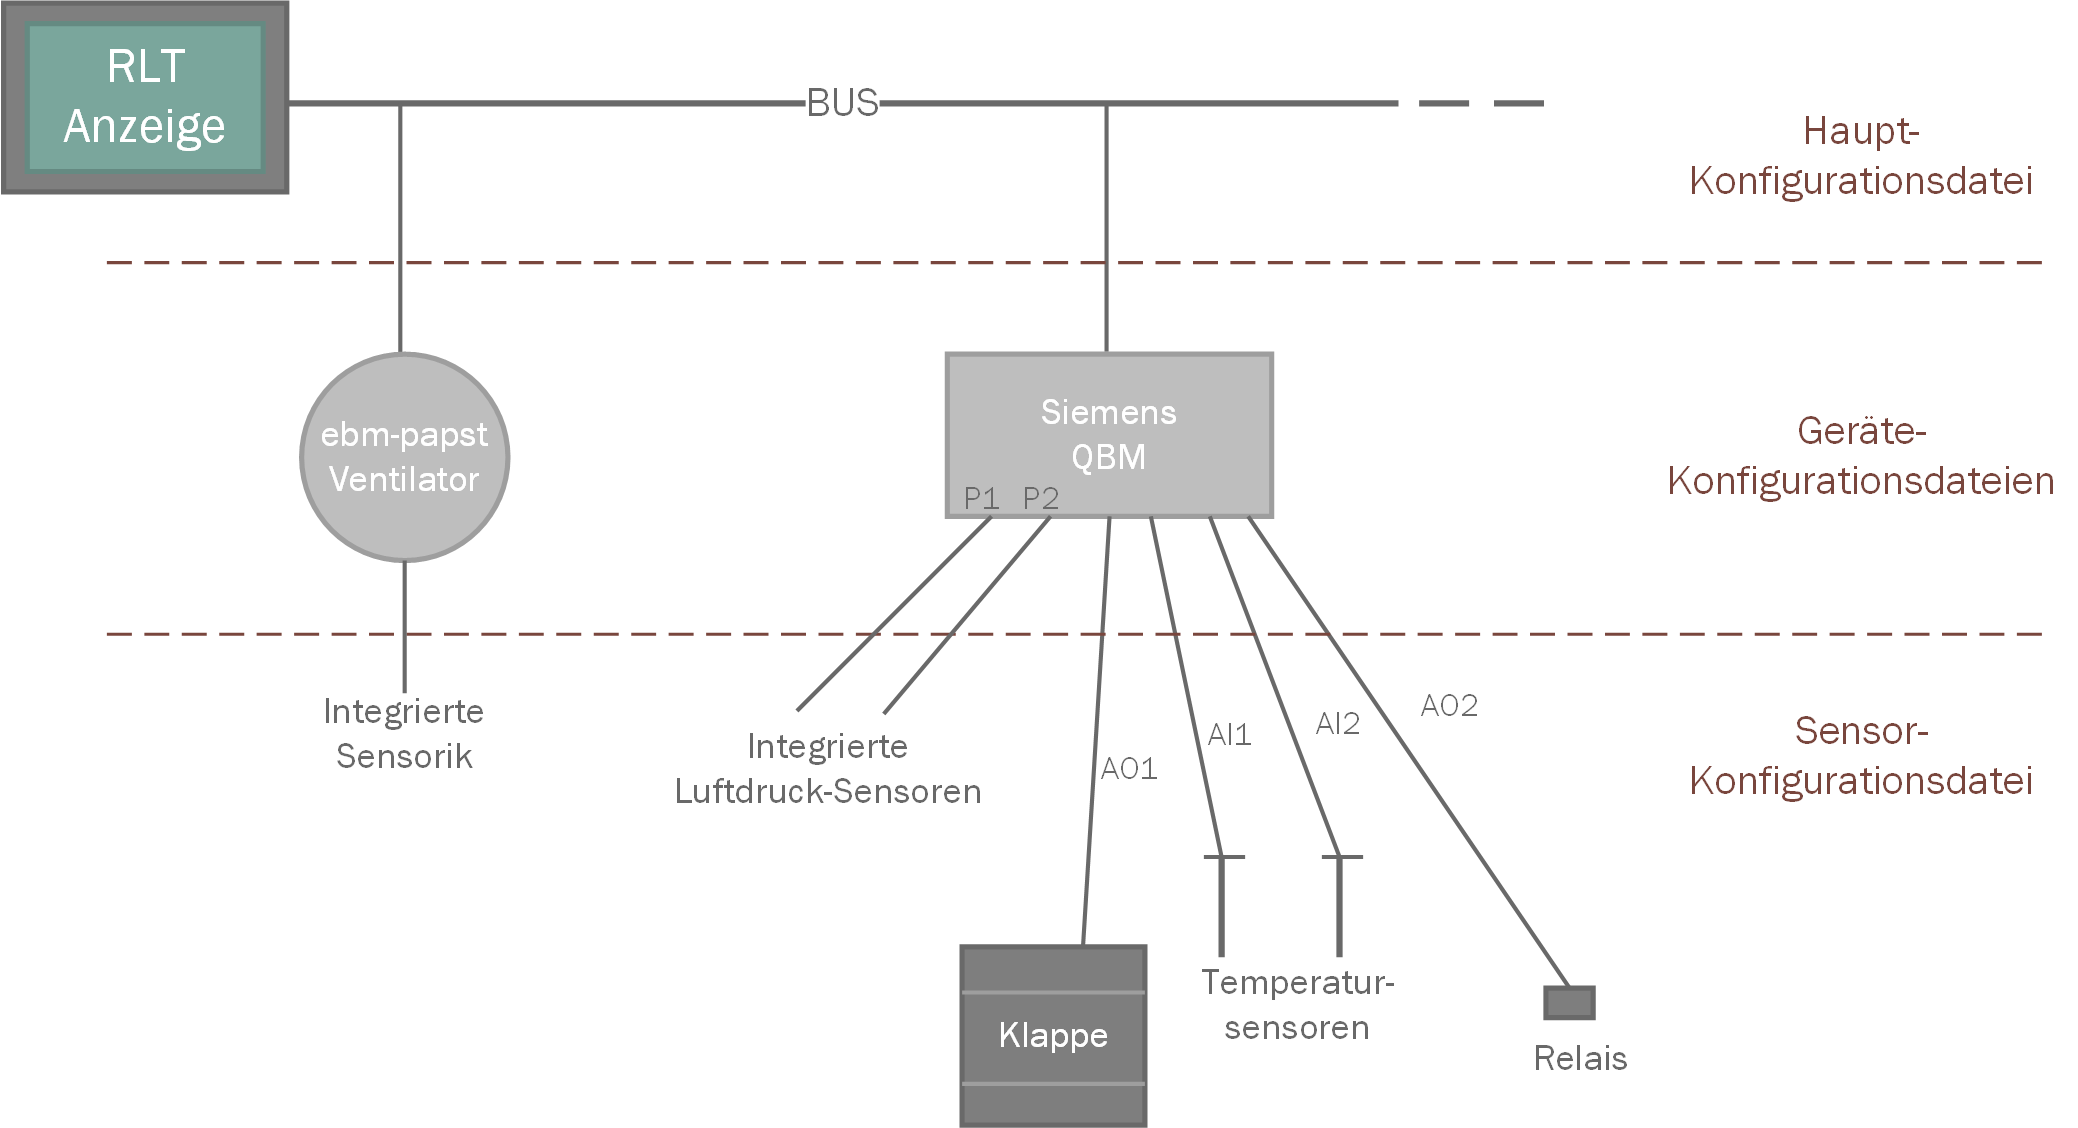
\includegraphics[width=\textwidth]{Komponenten_simpler_Aufbau_fuer_Dateikonzept}
	\caption{Vereinfachter Aufbau der Komponenten \label{fig:vereinfachter_aufbau_dateikonzept}}
\end{figure}

Es folgt eine nähere Beschreibung und Erklärung der drei Dateitypen:
%Fenkart fragen, ob ich bei den Geräten auf seinen Teil verweisen kann
% Wer beschreibt baud_rate, register, adresse, function code \ref{modbus_funktionsweise}

\begin{enumerate}

	\item \textbf{Sensor-Konfigurationsdatei} (\enquote{sensors.json}): Es gibt kein explizites Modbus Register, um die Maßeinheit eines Messwerts zu übertragen. Deswegen muss die Maßeinheit der unterschiedlichen Sensorik aus Datenblättern entnommen und jeweils zugeordnet werden. Dazu dient die Sensor-Konfigurationsdatei, welche eine Liste aller Sensoren (\zB bestimmte Temperatursensoren) mit der jeweils dazugehörigen Maßeinheit beinhaltet. Komponenten wie Ventilatoren haben integrierte Sensoren. Auch in diesem Fall kann für die Maßeinheit ein Eintrag in die \enquote{sensors.json} Datei gemacht werden. 
	
	Die einfache Ergänzung neuer Sensoren ist der Zweck der Sensor-Konfigurationsdatei. Diese muss nur dann verändert werden, wenn ein neuer Sensortyp, der noch nicht in der Sensor-Konfigurationsdatei steht, ergänzt wird. 
	
	Jeder Eintrag der Sensor-Konfigurationsdatei hat zwei Parameter, welche in in Tab. \ref{tab:sensors_json_parameter} zu sehen sind.
		
	\begin{table}[h]
		\caption{Parameter der Sensor-Konfigurationsdatei (\enquote{sensors.json})}
		\label{tab:sensors_json_parameter}
		\begin{tabular}{p{\dimexpr 0.15\textwidth-2\tabcolsep} p{0.5\textwidth} | p{0.3\textwidth}}
			\toprule
			\textbf{Name} & \textbf{Beschreibung} & \textbf{Beispiel} \\
			\midrule
			type & Der Sensorname, auf den später in der Haupt-Konfigurationsdatei unter \enquote{type} referenziert wird. &  
			\begin{jsonTable}
"type": "NI1000"
			\end{jsonTable} 
 			\\
			unit & Die Einheit des entsprechenden Sensors. (Diese muss auch in der Geräte-Konfigurationsdatei unter \enquote{units} vorhanden sein.) &  
			\begin{jsonTable}
"unit": "°C"
			\end{jsonTable} 
			\\
			\bottomrule
		\end{tabular}
	\end{table}
	
	Ein Beispiel für einen Eintrag der Sensor-Konfigurationsdatei ist folgend zu sehen:
	\begin{jsoncode}
{
	"type": "NI1000",
	"unit": "°C"
},
	\end{jsoncode}
	
	\item \textbf{Geräte-Konfigurationsdateien} (\zB \enquote{QBM97XX.json} oder \enquote{EBM.json}): Hier sind gerätespezifische Daten hinterlegt. Hauptsächlich welche Ausgabeports eine bestimmte Komponente (\zB ein Ventilator) besitzt, welche Einstellungen diese Ausgänge haben und \ggf welche Maßeinheiten die extern angeschlossenen Sensoren zurückgeben. 
	
	Weil in den \acs{rltanlagen} der Firma Bösch häufig die gleichen Komponenten verwendet werden, wurden spezielle Geräte-Konfigurationsdateien konzipiert. Diese Dateien können in der Haupt-Konfigurationsdatei beliebig oft referenziert werden, da sie einmalig für jedes Gerätemodell erstellt werden und nur selten Änderungen unterliegen. Das Hinzufügen einer neuen Geräte-Konfigurationsdatei ermöglicht zudem die einfache Integration einer neuen Komponente, beispielsweise eines Ventilators einer anderen Marke.
	
	Der Aufbau der Geräte-Konfigurationsdateien basiert auf einem \enquote{ports} Array. In dieses werden mithilfe der Parameter aus Tabelle \ref{tab:ports_array_parameter} die erforderlichen Informationen eingetragen.
	
	\begin{table}[H]
		\caption{Parameter im \enquote{ports} Array der Geräte-Konfigurationsdateien}
		\label{tab:ports_array_parameter}
		\begin{tabular}{p{\dimexpr 0.18\textwidth-2\tabcolsep} p{0.5\textwidth} | p{0.27\textwidth}}
			\toprule
			\textbf{Name} & \textbf{Beschreibung} & \textbf{Beispiel} \\
			\midrule
			port      	& Bezeichnung des Ausgabeports. Wird im Falle eines Geräts mit externer Sensorik (\zB Siemens QBM) in der Haupt-Konfigurationsdatei unter \enquote{port} referenziert. & 
			\begin{jsonTable}
"port": "AI1"
			\end{jsonTable} 
			\\
			register 	& !!!!!!!!!!!Das Register, welches vom Modbus ausgelesen werden soll (Bemerkung: Immer Dezimal, nicht HEX) & 
			\begin{jsonTable}
"register": 11
			\end{jsonTable} 
			\\
			function\_code 	& Modbus-Funktionscode, mit dem auf das vorherig angegebene Register zugegriffen werden soll: 3 für Input Register, 4 für Holding Register & 
			\begin{jsonTable}
"function_code": 3
			\end{jsonTable} 
			\\
			units 	& Array mit Unit-Objekten; Wird bei Ports weggelassen, bei denen die Werte nur von Python-Funktionen verwendet werden; In einem Objekt dieses Arrays werden folgende Parameter angegeben: „unit“, „scaling“; Funktionsweise / Zweck: Einheit wird mit dem „type“-Attribut zuerst aus der Sensor-Konfigurationsdatei herausgeholt und dann hier verglichen. Dann wird die Skalierung ausgelesen und der Wert aus dem Modbus damit multipliziert
			z. B. „type“ : „NI1000“ $\rightarrow$ „unit“ : „°C“ $\rightarrow$ „scaling“ : 0.1 $\rightarrow$ Ausgelesener Wert wird mit 0,1 multipliziert & 
			\begin{jsonTable}
"units": "[ ]"
			\end{jsonTable} 
			\\
			\bottomrule
		\end{tabular}
	\end{table}
	
	\begin{table}[H]
		\caption{Parameter im Unterarray \enquote{units}}
		\label{tab:pages_array_parameter}
		\begin{tabular}{p{\dimexpr 0.18\textwidth-2\tabcolsep} p{0.47\textwidth} | p{0.3\textwidth}}
			\toprule
			\textbf{Name} & \textbf{Beschreibung} & \textbf{Beispiel} \\
			\midrule
			unit      	& Die Einheit, welche aus „sensors.json“ referenziert wird & 
			\begin{jsonTable}
"unit": "°C"
			\end{jsonTable} 
			\\
			scaling 	& Skalierung des Messwertes (wird \zB verwendet, wenn der Messwert Kommastellen besitzt). Kann aus Datenblättern entnommen werden. & 
			\begin{jsonTable}
"scaling": 0.1
			\end{jsonTable} 
			\\
			\bottomrule
		\end{tabular}
	\end{table}
	
\begin{jsoncode}
{
	"port": "AI1",
	"register": 9,
	"function_code": 3,
	"units": [
	{
		"unit": "°C",
		"scaling": 0.1
	},
	{
		"unit": "mV",
		"scaling": 1
	}
	]
},
\end{jsoncode}
	
	\item \textbf{Haupt-Konfigurationsdatei} (\enquote{main\_config\_file.json}): Wie in Kapitel \ref{gui_design} beschrieben, werden zur übersichtlichen  Anzeige der Messwerte mehrere Abschnitte \bzw Seiten benötigt. Auf diesen Seiten werden jeweils sinngemäß Messwerte zusammengefasst. 
	
	Die Aufteilung der Seiten wird in der Haupt-Konfigurationsdatei gemacht. Dabei werden alle Seiten, die später auf der \acs{rltanzeige} angezeigt werden sollen, im \enquote{pages} Array definiert. Dazu werden unterschiedliche Parameter angegeben (siehe Tab. \ref{tab:pages_array_parameter}).
	
	% unterschiedliche anzahl der Komponenten

	\begin{table}[H]
		\caption{Parameter im \enquote{pages} Array der Haupt-Konfigurationsdatei}
		\label{tab:pages_array_parameter}
			\begin{tabular}{p{\dimexpr 0.15\textwidth-2\tabcolsep} p{0.45\textwidth} | p{0.35\textwidth}}
			\toprule
			\textbf{Name} & \textbf{Beschreibung} & \textbf{Beispiel} \\
			\midrule
			title      	& Beliebig auswählbarer Titel der Seite. & 
			\begin{jsonTable}
"title": "Allgemein"
			\end{jsonTable} 
			\\
			sources 	& Array aller Messwerte, die auf einer Seite angezeigt werden sollen. Die Parameter, die in einem Objekt dieses Arrays benutzt werden, sind in Tab. \ref{tab:sources_array_parameter} zu sehen. & 
			\begin{jsonTable}
"sources": "[ ]"
			\end{jsonTable} 
			\\
			\bottomrule
		\end{tabular}
	\end{table}
	
	\begin{table}[H]
		\caption{Parameter im Unterarray \enquote{sources}}
		\label{tab:sources_array_parameter}
			\begin{tabular}{p{\dimexpr 0.2\textwidth-2\tabcolsep} p{0.42\textwidth} | p{0.33\textwidth}}
			\toprule
			\textbf{Name} & \textbf{Beschreibung} & \textbf{Beispiel} \\
			\midrule
			port                & Ein Array mit den Quellen, aus denen der Messwert ausgelesen wird. Dabei wird meistens nur ein Objekt mit \enquote{id} des Geräts und \enquote{port} (siehe Tab. \ref{tab:devices_array_parameter})angegeben. In manchen Fällen werden mehrere Quellen für abgeleitete Messwerte benötigt (siehe Kapitel \ref{python_functions}). In dem Fall werden dem Array weitere Objekte hinzugefügt. &  
			\begin{jsonTable}
"port": [
	{ "QBM1": "AI1" }
]
			\end{jsonTable} 
			\\
			description         & Beliebig auswählbare Bezeichnung für einen Messwert, die auf der \acs{rltanzeige} später angezeigt wird. & 
			\begin{jsonTable}
"description": "Temperatur Zuluft"
			\end{jsonTable}  
			\\
			python\_function    & Optionaler Parameter, der angegeben wird, wenn der jeweilige Messwert abgeleitet berechnet werden muss. Weitere Erklärung in Kapitel \ref{python_functions}. & 
			\begin{jsonTable}
"python_function": "relay_position"
			\end{jsonTable} 
			\\
			additional\_info    & Optionaler Parameter, der angegeben wird, falls bei der Python Funktion zusätzliche Informationen braucht. Weitere Erklärung in Kapitel \ref{python_functions}. & 
			\begin{jsonTable}
"additional_info": { "switching_voltage": 5 }
			\end{jsonTable} 
			\\
			\bottomrule
		\end{tabular}
	\end{table} 
		
	Ein Beispiel für einen Seiteneintrag im \enquote{pages} Array ist folgend zu sehen:
	
%	\jsonfile[firstline=2, lastline=12]{Code/main.py}
	\begin{jsoncode}
"pages": [
	{
		"title": "Temperaturen QBM1",
		"sources": [
		{
			"port": [{ "QBM1": "AI1" }],
			"description": "Temperatur 1"
		},
		{
			"port": [{ "QBM1": "AI2" }],
			"description": "Temperatur 2"
		},
		...
		{
			"port": [{ "QBM1": "AO1" }],
			"description": "Klappe",
			"python_function": "flap_position"
		}
		]
	},
	...
]
	\end{jsoncode}
	
		
	Parallel zum \enquote{pages} Array \bzw auf der gleichen Ebene der Haupt-Konfigurationsdatei gibt es ein \enquote{devices} Array. Darin werden die Komponenten der \acs{rltanlage} angegeben, von denen Messwerte ausgelesen werden sollen.
	
	\begin{table}[H]
		\caption{Parameter im \enquote{devices} Array}
		\label{tab:devices_array_parameter}
		\begin{tabular}{p{\dimexpr 0.2\textwidth-2\tabcolsep} p{0.43\textwidth} | p{0.32\textwidth}}
			\toprule
			\textbf{Name} & \textbf{Beschreibung} & \textbf{Beispiel} \\
			\midrule
			device     	&  & Bsp \\
			id         	&  & Bsp \\
			baud\_rate	&  & Bsp \\
			mbaddress	&  & Bsp \\
			parity	&  & Bsp \\
			stop\_bits	&  & Bsp \\
			zero\_based	&  & Bsp \\
			sensors	&  & Bsp \\
			\bottomrule
		\end{tabular}
	\end{table} 
	
\end{enumerate}

%Bedienungsanleitung für Servicetechniker erwähnen
Dabei ist zu beachten:
Der Techniker bekommt einen Ordner, darin findet sich direkt eine Vorlage für die \enquote{main\_config\_file.json}-Datei, welche im Normalfall die einzige Datei sein sollte, die vom Techniker bearbeitet bzw. verändert wird.
In einem Unterordner (\enquote{devices}) sind dann die Geräte-Konfigurationsdateien und die Sensor-Konfigurationsdatei. Diese Dateien müssen, wie oben erwähnt, nur verändert werden, wenn noch nie verwendete Geräte oder Sensorik, wie z.B. eine neue Art von Ventilator oder Sensor, in der RLT-Anlage verbaut werden.

Beispiel zu allen Dateitypen im Anhang!!!




